\documentclass[10pt]{examdesign}
\usepackage{amsmath}
\usepackage{enumitem}
\usepackage{amsfonts}
\usepackage{pgfplots}
\usepackage{pifont}
\usepackage{graphicx}
\usepackage{fancyhdr}
\usepackage{cancel}
\usepackage{graphicx}

\SectionFont{\large\sffamily}
\Fullpages
\ContinuousNumbering
\usepackage{ulem}
\ProportionalBlanks{2}


\DefineAnswerWrapper{}{}
\NumberOfVersions{2}
%\IncludeFromFile{foobar.tex}
\examname{Semester 2 Exam}
\class{ {\Large Physics}}

\def \namedata {Name: \hrulefill\\ 
	Date: \hrulefill \\
	Period: \hrulefill
	
}




\begin{document}




\begin{multiplechoice} [title={Multiple Choice (3 Points Each)},
	rearrange=yes]
	\textit{Choose the best answer to each question.} 
	
	\begin{question}
	A lens has a focal length of -5 cm.  Which statement must be true?
		\choice{The image must be real.}
		\choice{The image must be inverted.}
		\choice[!]{The image must be smaller.}
		\choice{The image must be larger.}
	\end{question}



	\begin{question}
	A penny is placed in the bottom of a cup, and the cup is placed so that the penny is just outside the person's view, as shown in the picture.  If the cup is carefully filled with water without causing the penny to move, what will happen?
		
	\begin{center} 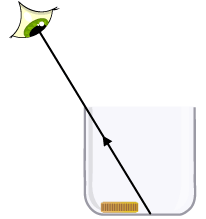
\includegraphics[width=1.25in]{penny.png} \end{center}
	
		\choice[!]{As the water level rises the penny will become visible due to refraction.}
		\choice{As the water level rises the penny will remain out of the person's view.}
		\choice{as the water level rises reflections of the penny will become visible on the surface of the water.}
		\choice{As the water level rises, the penny will become completely invisible.}
\end{question}

\begin{block}
	
	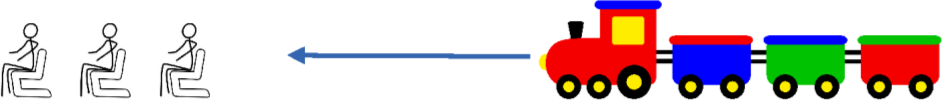
\includegraphics[width=5in]{train.png} 
	
	
	\begin{question}
		A train is approaching a train station where several students are sitting in chairs, as shown above.  If the train's whistle has a frequency of 700 Hz, the frequency the people hear is - 
		\choice[!]{Greater than 700 Hz} 
		\choice{Exactly 700 Hz}
		\choice{Less than 700 Hz}
		\choice{Each person hears a different frequency.}
	\end{question}
\end{block}


\begin{question}
	The number of times that a wave repeats itself in one second is known as its - 
	\choice{Wavelength}
	\choice{Amplitude}
	\choice[!]{Frequency}
	\choice{Period}
	
	\end{question}

	\begin{question}
	Kinetic Energy is best defined as - 
	\choice{Stored Energy}
	\choice{Electrical Energy}
	\choice{Thermal Energy}
	\choice[!]{Motion Energy}
	\end{question}
	
	\begin{question}
	The energy stored in a spring when it is stretched is called - 
	\choice[!]{Elastic Potential Energy}
	\choice{Gravitational Potential Energy}
	\choice{Electrostatic Potential Energy}
	\choice{Rotational Potential Energy}
	\end{question}
	
	\begin{question}
	A planet is found that is the exact same mass as Earth, and has all the conditions needed to support life, (oxygen, water, sunlight, etc) but there is no life on the planet.  An astronaut plants some grass and drops off some cows and bull.  Over the next thousand years, the grass grows and the cows reproduce.  If no other trips are made to visit the planet, the total mass of this planet (including the mass of the cows and the grass)
		\choice{Increases as the grass grows and the cows reproduce.}
		\choice[!]{Remains constant due to the law of conservation of mass.}
		\choice{Decreases due to the cows eating the grass.}
		\choice{Could increase, decrease, or remain the same depending on the final number of cows and total amount of grass after 1000 years.}
	\end{question}

	\begin{question}
	A pendulum of length $ \ell $ has a period of 1 second.  What would the period of a pendulum of length $ 3\ell $ be?
	\choice{3 seconds}
	\choice[!]{$\sqrt{3}$  seconds}
	\choice{$\frac{1}{\sqrt{3}}$ seconds}
	\choice{27 seconds}
	
	\end{question}


	\begin{question}
	A 3 kg block hangs from a spring that is attached to the ceiling of an elevator.  As the elevator accelerates upward, the spring - 
	\choice[!]{Gets longer}
	\choice{Gets shorter}
	\choice{Remains the same length}
	\choice{It cannot be determined without knowing the spring constant and the acceleration of the elevator.}
	\end{question}

	\begin{question}
	In the 1998 film \textit{Armageddon}, Bruce Willis is hired by NASA to detonate a nuclear bomb inside an asteroid that is on a collision course for earth.  In real life, this plan would be - 
	\choice{a good idea because it would destroy the asteroid.}
	\choice{a good idea because a nuclear blast at the center of the asteroid would deflect it away from the earth.}
	\choice[!]{a bad idea, because the center of mass of the asteroid would continue to move in the same direction.  Instead of one large impact there would be thousands of smaller impacts all over the world.}
	\choice{a bad idea because a nuclear bomb in space could kill everyone on Earth.}	
	\end{question}


	\begin{question}
	A wheel spins three times.  What is the angle (in radians) that the wheel has traveled?
	\choice{1080 radians}
	\choice[!]{$6\pi$ radians}
		\choice{$3\pi$ radians}
			\choice{3 radians}
	\end{question}

\begin{block}
	
	\textbf{The following two questions refer to the following information:} 
	The picture below shows an overhead view of China's Z-20 Anti-submarine helicopter.  Two points have been labeled A and B.  
	
	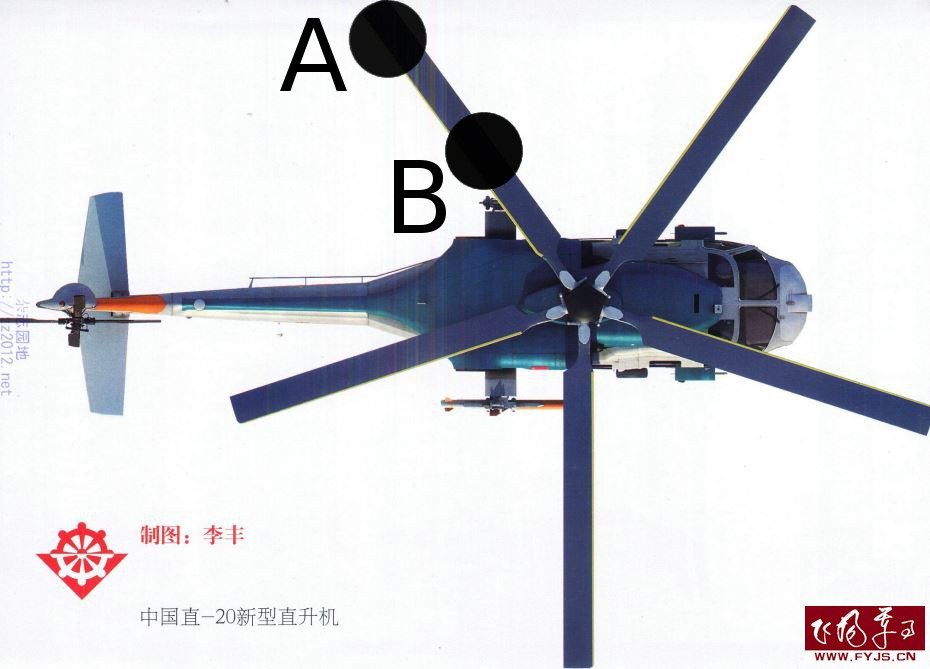
\includegraphics[height=3cm]{heli.jpg}
	
	
	
	\begin{question}
		When the helicopter blades are rotating, which point has a greater \underline{angular velocity ($\omega$)}?
		
		\vspace{0.1in}
		
		\choice{A}
		\choice{B}
		\choice[!]{They both have the same angular velocity}
		\choice{It is impossible to tell.}
	\end{question}
	
	\begin{question}
		When the helicopter blades are rotating, which point has a greater \underline{linear velocity (v)}?
		
		\vspace{0.1in}
		
		\choice{A}
		\choice{B}
		\choice[!]{They both have the same angular velocity}
		\choice{It is impossible to tell.}
	\end{question}
	
	
	
\end{block}

\begin{block}
	
	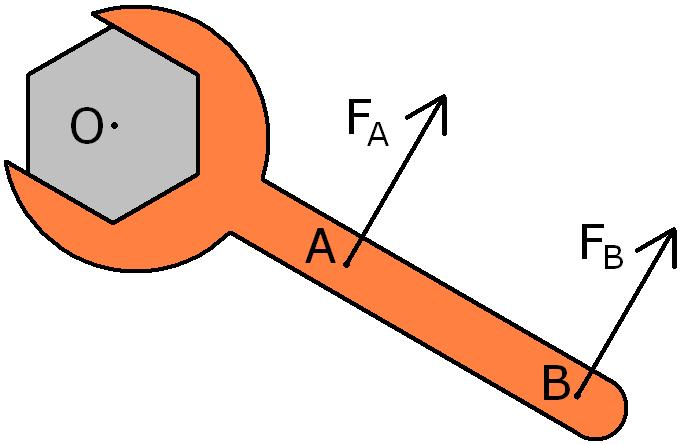
\includegraphics[height=3cm]{wrench.png}

	
\begin{question}

You are attempting to loosen a bolt from your car by putting a force on a wrench, as shown in the picture.   You can choose to put a force on the wrench at point A or at point B.  If both the forces are the same magnitude, which force is more effective in loosening the bolt?
\choice{Force A is more likely to turn the bolt because the force is applied closer to the bolt.}
\choice{Force A is more likely to turn the bolt because $\frac{F_A}{r}$ is greater than $\frac{F_B}{r}$.}
\choice{Force B is more likely to turn the bolt because FB has a larger magnitude.}
\choice[!]{Force B is more likely to turn the bolt because it produces a greater torque.}
\choice{Both forces will turn the bolt in the same manner because the magnitude of both forces is the same.}
\end{question}
\end{block}

\begin{question}
Bats use ultrasonic sounds of 25000 Hz to find bugs by echolocation.  A bat is flying 7 m/s to the right.  A bug is to the right of the bat, and hears a sound of 21500 Hz.  Which is the best description of the motion of the bug?
\choice{To the left, faster than 7 m/s.}
\choice[!]{To the right, faster than 7 m/s.}
\choice{To the left, slower than 7 m/s.}
\choice{To the right, slower than 7 m/s.}
\end{question}

\begin{question}
	While you are driving on the highway, a bug collides with the windshield of your car.  The impulse on the bug is - 
	\choice [!]{equal to the impulse on the car and in the opposite direction.}
	\choice {less than the impulse on the car and in the same direction.}
	\choice {greater than the impulse on the car and in the opposite direction.}
	\choice {equal to the impulse on the car and in the same direction. }
\end{question}


\begin{question}
	An object is placed 4 cm to the left of a lens.  A real image forms 4 cm to the right of the lens.  What is the focal length of the lens?
		\choice{1 cm}
		\choice[!]{2 cm}
		\choice{3 cm}
		\choice{4 cm}
\end{question}

\begin{question}
 Corn Syrup has an index of refraction of 1.5044.  What is the speed of light in corn syrup?
 	\choice{$4.513 \times 10^8$ m/s}
 	\choice{$2.998 \times 10^8$ m/s}
 	\choice[!]{$1.994 \times 10^8$ m/s}
 	\choice{$5.01 \times 10^{-9}$ m/s}
\end{question}

\begin{question}
	In marching band, Emily plays an \textit{A} on her clarinet (f = 440 Hz) as she marches forward at 2 m/s.  What frequency would a spectator in the stands hear? 
	\choice{445.178 Hz}
	\choice[!]{442.581 Hz}
	\choice{437.449 Hz}
	\choice{432.273 Hz}
\end{question}

\begin{question}
	An ocean wave moves toward the shore at 2m/s.  It has a period of 5 seconds.  What is its wavelength?
	\choice[!]{0.4 m}
	\choice{1 m}
	\choice{2.5 m}
	\choice{10m}	
\end{question}



\begin{question}
	What is the kinetic energy of a 1000 kg car that travels at 20 m/s?
	\choice{10000 J}
	\choice{20000 J}
	\choice[!]{200000 J}
	\choice{400000 J}
\end{question}

\begin{question}
	An Eagle drops a clam from a height of 43 m in order to break its shell open.  What is the speed of the clam as it hits the ground?
	\choice{20.539 m/s}
	\choice[!]{29.046 m/s}
	\choice{843.66 m/s}
	\choice{It cannot be determined without knowing the mass of the clam.}
	
\end{question}

	\begin{question}
	A hunting whale is swimming at 6 m/s when it catches a sleeping giant squid of the same mass in its mouth.  Immediately after catching the squid, how fast will the two be moving?
	\choice {12 m/s}
	\choice {6 m/s}
	\choice [!]{3 m/s}
	\choice {It is impossible to tell. }
\end{question}



\begin{question}
	A pendulum has a length of 0.37m.  What is its period?
	\choice{0.237 s}
	\choice[!]{1.220 s}
	\choice{2.441 s}
	\choice{3.7 s}
\end{question}


\begin{question}
	A spring has 0.4 J of elastic potential energy when it is stretched 0.03m.  What is the spring constant of the spring?
	\choice{13.333 N/m}
	\choice{26.667 N/m}
	\choice{133.33 N/m}
	\choice{888.888 N/m}
\end{question}


\begin{block}
		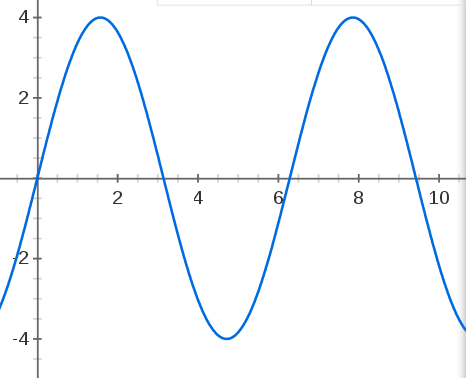
\includegraphics[height=4cm]{wave2.png}
	
\begin{question}
	What is the approximate amplitude of the wave shown above?
\choice{8 meters}
\choice{6.28 meters}
\choice{4 meters}
\choice{3.14 meters}
	\end{question}

\end{block}


\begin{question}
A regulation basketball (m=0.625 kg) and a 12-pound bowling ball (m=5.44311 kg) are allowed to roll down a ramp.  The moment of inertia of a solid sphere is $I = \frac{2}{5} mr^2$, and the moment of inertia for a hollow sphere is $I = \frac{2}{3} mr^2$.  Which object reaches the bottom of the ramp first?
\choice{The Basketball}
\choice{The Bowling Ball}
\choice{They both reach the bottom at the same time.}
\choice{It cannot be determined without knowing the angle of the ramp.}
\end{question}



\begin{question}
	A dog is at the back of an empty boat when he sees an interesting fish jump near the front of the boat.  The dog runs 4 meters east, to the front of the boat, then stops.  The dog has a mass of 30kg, and the boat has a mass of 60 kg.  If there is no friction between the boat and the water, how far does the boat move? 
	\choice{1 m}
	\choice[!]{2 m}
	\choice{3 m}
	\choice{4 m}
\end{question}


	\begin{question}
	Which of the following is the best example of an \textbf{\underline{inelastic}} collision.
	\choice{William dribbles a basketball.}
	\choice{Diego kicks a soccer ball.}
	\choice[!]{Victor throws his gum and it sticks to the wall.}
	\choice{Martin punches the wall and makes a hole in it.}
\end{question}
\end{multiplechoice}



\begin{shortanswer}[title={Lab Question (10 Points)}, rearrange=NO]
	
	

		\textit{This question requires you to collect data at a lab station.}  Go to a lab station that is unoccupied. \vspace{0.1in}
		
		Use a light source such as your phone or a calculator to create an image.  
		
		\vspace {0.1in} Measure the distance from the object to the lens (o) and the distance from the lens to the screen (i). 
		
	\begin{question}		The focal length of this lens is closest to - 
		\begin{enumerate}
			\item 5cm
			\item 10 cm
			\item 15 cm
			\item 20 cm
	
		\end{enumerate} 
		\vspace{2in}
	\end{question}
	
	
	
\end{shortanswer}


\begin{multiplechoice} [title={Survey Questions (1 Point Each)},
	rearrange=no]
	\textit{Please answer the following questions.  Your answers to these questions will not affect your score, they will only be graded for completion.  } 

\begin{question}
	 The instructor presented the material clearly.
\\a) Strongly Agree	b) Agree	c) Neutral	d) Disagree	e) Strongly Disagree
\end{question}

\begin{question}
 The instructor presented all the skills needed to be successful in the course.
\\a) Strongly Agree	b) Agree	c) Neutral	d) Disagree	e) Strongly Disagree
\end{question}

\begin{question}
The instructor presented material in a way that was easy for me to understand.
\\a) Strongly Agree	b) Agree	c) Neutral	d) Disagree	e) Strongly Disagree
\end{question}
\begin{question}
The instructor graded assignments and exams fairly. 
\\a) Strongly Agree	b) Agree	c) Neutral	d) Disagree	e) Strongly Disagree
\end{question}
\begin{question}
The instructor was helpful when I asked him questions.
\\a) Strongly Agree	b) Agree	c) Neutral	d) Disagree	e) Strongly Disagree
\end{question}
\begin{question}
The instructor cared about me as a person.
\\a) Strongly Agree	b) Agree	c) Neutral	d) Disagree	e) Strongly Disagree
\end{question}
\begin{question}
The amount of work in this course was - 
\\a) Way too much	b) Too much	c) Just Right	d) Too little	e) Way too little.
\end{question}
\begin{question}
In a typical week, how much time did you spend on homework for this class?
\\a) 0-1 hours	b) 1-2 hours	c) 2-3 hours	d) 3-4 hours 	e) More than 4 hours.
\end{question}
\begin{question}
Rather than immediately giving answers, the instructor gave me opportunities to correct myself.
\\a) Always	b) Often		c) Sometimes	d) Rarely	e) Never
\end{question}
\begin{question}
The instructor is  professional and courteous.
\\a) Always	b) Often		c) Sometimes	d) Rarely	e) Never
\end{question}
\begin{question}
I expect to get a passing grade in this course
\\a) Definitely	b) Probably	c) Neutral	d) Probably Not	e) Definitely Not.
\end{question}
\begin{question}
The pace of the course was - 
\\a) Way Too Slow	b) Somewhat Too Slow	c) Just Right	d) Somewhat Too Fast	e) Way Too Fast.
\end{question}
\begin{question}
Would you recommend this instructor to a friend? 
\\a) Definitely	b) Probably	c) Neutral	d) Probably Not	e) Definitely Not.
\end{question}
\begin{question}
Overall, how would you rate this course? 
\\a) Great		b) Good		c) Average	d) Below Average	e) Awful
\end{question}
\begin{question}
Overall, how would you rate this instructor?
\\a) Great		b) Good		c) Average	d) Below Average	e) Awful
\end{question}

\begin{question}
Please include any other comments you have about this course or instructor in the lined area on your scantron.
\end{question}

\end{multiplechoice}

\end{document}


